\documentclass[../bccalc.tex]{subfiles}
\graphicspath{{\subfix{../figures/}}}
\begin{document}
\chapter{Applications of Differentiation}
\section{Definition of the Derivative Meets Derivative Rules}
\begin{example}
    Evaluate the following by recognizing that the given limit represents a derivative. 
    \[ \lim_{h\to 0} \frac{2(x+h)^3-2x^3}{h} \]

    We know $f(x)=2x^3$, so the derivative is trivial from this.
\end{example}

\ex Evaluate the following by recognizing the given limit represents a derivative. 

$\lim_{h\to 0} \frac{\cos (5(x+h)) - \cos(5x)}{h}$

\ex Evaluate the following by recognizing the given limit represents a derivative. 

$\lim_{h\to 0} \frac{\sin \left(\frac{\pi}{6}+h\right)-\frac{1}{2}}{h}$

\section{Related Rates}
We have previously learned the Chain Rule and this allows us to use implicit differentiation for related rates.

\begin{example}
    Suppose $y=5x^2-6x+2$. Find $\frac{dy}{dt}$ when $x=4$, given that $\frac{dx}{dt}=2$ when $x=4$.

    We are taking the derivative of $y$ with respect to $t$.

    We get $\frac{dy}{dt}(y=5x^2-6x+2)=\frac{dy}{dt}=10x\frac{dx}{dt}-6\frac{dx}{dt}$.

    Plug this in to get $68$ as the answer.
\end{example}

\begin{example}
    A pebble is dropped into a calm pond, causing ripples in the shape of concentric circles. The radius of the outer ripple is increasing at a constant rate of 1 ft/sec. When the radius is 4 ft, find the rate at which the area of the disturbed water is changing.

    We have to do the derivative of $A=\pi r^2$, the circle formula.

    This is $2\pi r \frac{dr}{dt}$. Plug in numbers to get $8 \pi$ ft$^2$/sec
\end{example}

\ex Water runs out of a conical tank at the constant rate of 2 cubic feet per minute. The radius at the top of the tank is 5 feet, and the height of the tank is 10 feet. How fast is the water level sinking when the water is 4 feet deep?
\pagebreak
\begin{example}
    A fish is reeled in at a rate of 2 ft/sec from a bridge 16 ft above the water. At what rate is the angle between the line and the water changing when there are 20 ft of line out?

    If we let $x$ be the distance from the fish to the person, then we know $\frac{dx}{dt} = -2$.

    We are trying to find $\frac{d\theta}{dt}$.

    Using trig, we can find $\tan \theta = 16x^{-1}$.

    The derivative gives $\sec^2 \theta\frac{d\theta}{dt}=-16x^{-2}\frac{dx}{dt}$.

    Plugging in numbers and solving for $\frac{d\theta}{dt}=\frac{2}{25}$ rad/s.
\end{example}

\ex A man 6 ft tall walks at a rate of 5 ft/sec away from a lightpole 16 ft tall. 

(a) At what rate is the tip of his shadow moving when he is 10 ft from the base of the light?

(b) At what rate is the length of his shadow moving when he is 10 ft from the base of the light?

\ex A trough is 10 ft long and 6 ft across the top. Its ends are isosceles triangles with an altitude of 4 ft. If water is being pumped into the trough at 9 ft$^3$/sec, how fast is the water level rising when the water is 2 ft deep?

\section{Extrema on an Interval}
\begin{definition}[Definition of Extrema]
    Let $f$ be defined on an interval $I$ containing $c$.
    \begin{enumerate}
        \item $f(c)$ is the minimum of $f$ on $I$ if $f(c)\leq f(x)$ for all $x$ in $I$.
        \item $f(c)$ is the maximum of $f$ on $I$ if $f(c)\geq f(x)$ for all $x$ in $I$.
    \end{enumerate}

    The minimum and maximum of a function on an interval are the extreme values or extrema of the function on the interval. The minimum and maximum of a function on an interval are also called the absolute minimum and absolute maximum, or the global minimum and global maximum, on the interval.
\end{definition}

\begin{definition}[Relative Extrema]
    \begin{enumerate}
        \item If there is an open interval containing $c$ on which $f(c)$ is a maximum, then $(c, f(c))$ is called a relative maximum of $f$, or you can say that $f$ has a relative maximum at $(c,f(c))$.
        \item If there is an open interval containing $c$ on which $f(c)$ is a minimum, then $(c,f(c))$ is called a relative minimum on $f$, or you can say that $f$ has a relative minimum at $(c,f(c))$.
    \end{enumerate}

    The relative maximum and relative minimum points are sometimes called local maximum and local minimum points, respectively.
\end{definition}
\pagebreak
\begin{example}
    In the figure, wind where $f$ has an absolute maximum, absolute minimum, relative maximum, and relative minimum on the interval $[-2,4]$.
    \begin{center}
        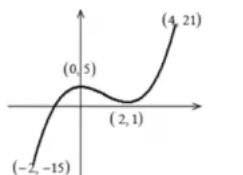
\includegraphics[width=0.3\textwidth]{3.1.1.PNG}
    \end{center}
    Absolute maximum at 4, absolute minimum at $-2$, relative maximum at 0, relative minimum at 2.
\end{example}

\begin{definition}[Critical Number and Critical Point]
    Let $f$ be defined at $c$. If $f'(c)=0$ or if $f$ is not differentiable at $c$, then $c$ is a critical number of $f$ and the point $(c,f(c))$ is a critical opint of $f$.
\end{definition}

\begin{theorem}
    Relative extrama occur only at critical numbers.
\end{theorem}

\begin{example}
    In the following, name the maximum and minimum points.
    \begin{center}
        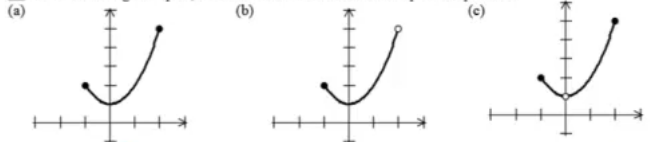
\includegraphics[width=0.7\textwidth]{3.1.2.png}
    \end{center}

    (a) Minimum at 0, maximum at 2 

    (b) Minimum at 0, no maximum 

    (c) no minimum, maximum at 2
\end{example}

Continuity is needed to guarantee a maximum and minimum.

\begin{theorem}[Extreme Value Theorem]
    If $f$ is continuous on a closed interval $[a,b]$, then $f$ attains an absolute maximum value $f(c)$ or an absolute minimum value $f(d)$ for some numbers $c$ and $d$ in $[a,b]$.
\end{theorem}

Guidelines for Finding Extrema on a Closed Interval - Candidates Test 

To find the extrema of a continuous function $f$ on a closed interval $[a,b]$, we used the following steps:
\begin{enumerate}
    \item Find $f'(x)$ and the critical numbers of $f$ in $[a,b]$.
    \item Evaluate $f$ at each critical number in $(a,b)$.
    \item Evaluate $f$ at each endpoint in $[a,b]$.
    \item The least of these values is the minimum. The greatest is the maximum.
\end{enumerate}

\begin{example}
    Find the absolute maximums and minimums of $f$ on the given closed interval, and state where these values occur.

    (a) $f(x)=3x^2-24x-1 \qquad [-1,5]$

    $f'(x)=0$ when $x=4$.

    $f$ has an absolute maximum of 26 at $x=-1$ and $f$ has an absolute minimum of $-49$ at $x=4$.

    (b) $f(x)=6x^3-6x^4+5 \qquad [-1,2]$.

    $f'(x)=18x^2-24x^3=0$.

    $x=0$ and $x=3/4$.

    $f$ has an absolute maximum of 5.6328 at $x=3/4$ and an absolute minimum of $-43$ at $x=2$.
\end{example}

\ex Same as above for $f(x)=3x^{2/3}-2x+1 \qquad [-1,8]$

\ex Same as above for $f(x)=\sin^2 x+\cos x\qquad [0,2\pi]$



\section{Mean Value Theorem and Rolle's Theorem}

\section{Increasing and Decreasing Functions and the First Derivative Test}

\section{Concavity and the Second Derivative}

\section{Second Derivative Test}

\section{Graphs of f, f', and f''}
\end{document}